\documentclass{article}
\usepackage{hyperref}
\usepackage{listings}
\usepackage{color}
\usepackage{xcolor}
\usepackage{geometry}
\usepackage{graphicx}
\usepackage{amsmath}
\usepackage{caption}
\usepackage{subcaption}
\geometry{margin=1in}
\pdfminorversion=6

\newcommand\TODO[1]{\textcolor{red}{TODO: #1}}

\newcommand\header[2]{
    \begin{center}
        {\large
        UCSD CSE 168 Assignment #1: \\
        \vspace{0.3cm}
        \Large
        #2}
    \end{center}
}

\definecolor{dkgreen}{rgb}{0,0.6,0}
\definecolor{gray}{rgb}{0.5,0.5,0.5}
\definecolor{mauve}{rgb}{0.58,0,0.82}
\lstset{frame=tb,
        aboveskip=3mm,
        belowskip=3mm,
        showstringspaces=false,
        columns=flexible,
        basicstyle={\small\ttfamily},
        numbers=none,
        numberstyle=\tiny\color{gray},
        keywordstyle=\color{blue},
        commentstyle=\color{dkgreen},
        stringstyle=\color{mauve},
        breaklines=true,
        breakatwhitespace=true,
        tabsize=2
}

\hypersetup{colorlinks=true}


\begin{document}

\header{2}{Triangles and acceleration structures}

In this homework, we are going to make your renderer capable of rendering more complex scenes.
The most commonly used primitive in computer graphics is a triangle. We will extend your renderer to handle objects that are made of \emph{triangle meshes}. Looping over each triangle is very slow. A scene can easily contain millions or billions of triangles (for example, in the movie Moana, \href{https://www.disneyanimation.com/resources/moana-island-scene/}{a scene of its island} contains more than 15 billion primitives). We will need something better.

For this homework, we will move to the second book of the Ray Tracing in One Weekend series: \href{https://raytracing.github.io/books/RayTracingTheNextWeek.html}{Ray Tracing - The Next Week (RTNW)}. As usual, we take huge inspirations from Wojciech Jarosz's \href{https://cs87-dartmouth.github.io/Fall2022/assignments.html}{CS 87/287 at Dartmouth}.

\section{Intersection with a single triangle}
Like our previous homework, let's start with rendering a single triangle. There are many ways to do it with different degrees of efficiency. The RTNW book did not provide information about triangles, but you can easily find some online. The \href{https://en.wikipedia.org/wiki/M%C3%B6ller%E2%80%93Trumbore_intersection_algorithm}{Moller-Trumbore intersection algorithm} described in the Wikipedia page is useful. The \href{https://www.pbr-book.org/3ed-2018/Shapes/Triangle_Meshes#TriangleIntersection}{PBRT book} contains more details.
Or you can just google ray-triangle intersection.
Feel free to copy paste any code.

Go to \lstinline{hw2.cpp} and look at the function \lstinline{hw_2_1}. Using the camera parameters provided (\lstinline{lookfrom = (0, 0, 0), lookat = (0, 0, -1), up = (0, 1, 0), vfov = 45}), render a triangle read from the command line arguments (we have parsed them for you). If your ray hits a triangle, outputs its barycentric coordinates (for a triangle $p_0, p_1, p_2$, a point inside the triangle can be represented as $p = w p_0 + u p_1 + v p_2$, where $(w, u, v)$ is the barycentric coordinate and $w = 1 - u - v$). Otherwise, if the ray does not hit anything, return $(0.5, 0.5, 0.5)$. To have consistency with our homework 1 code, let's do antialiasing. We have parsed the \lstinline{-spp} argument for you too.

To see your results, type the following in the terminal:
\begin{lstlisting}[language=bash]
  ./torrey -hw 2_1 0  1 -3  -1 -1 -3  1 -1 -3
  ./torrey -hw 2_1 0  3 -4  -1 -2 -5  5 -1 -3
  ./torrey -hw 2_1 0 -3  1  -1  1 -4  1  1 -4
\end{lstlisting}

\begin{figure}[ht]
    \centering
    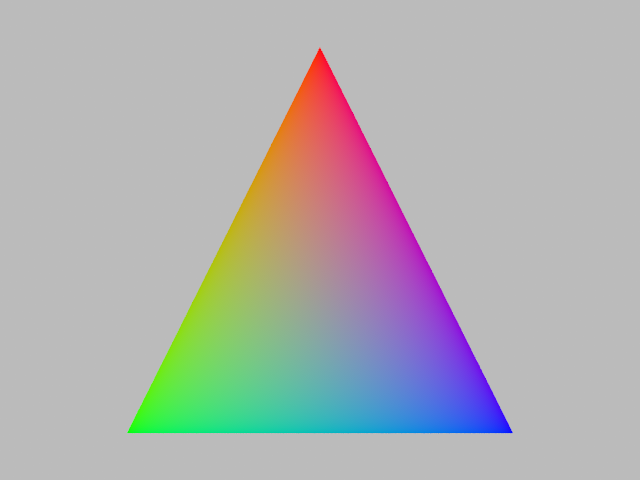
\includegraphics[width=0.3\linewidth]{imgs/hw_2_1a.png}
    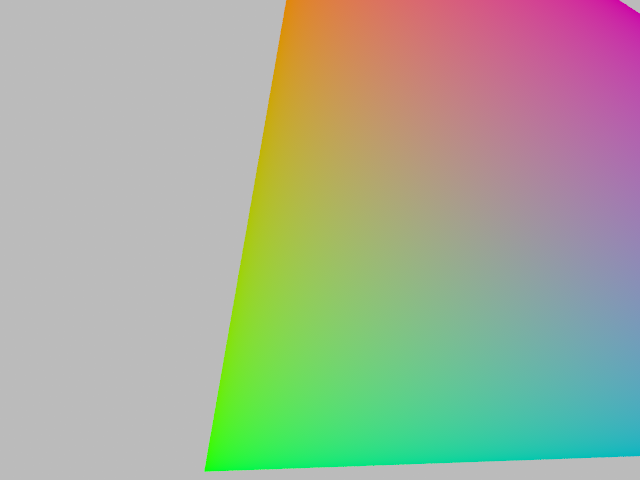
\includegraphics[width=0.3\linewidth]{imgs/hw_2_1b.png}
    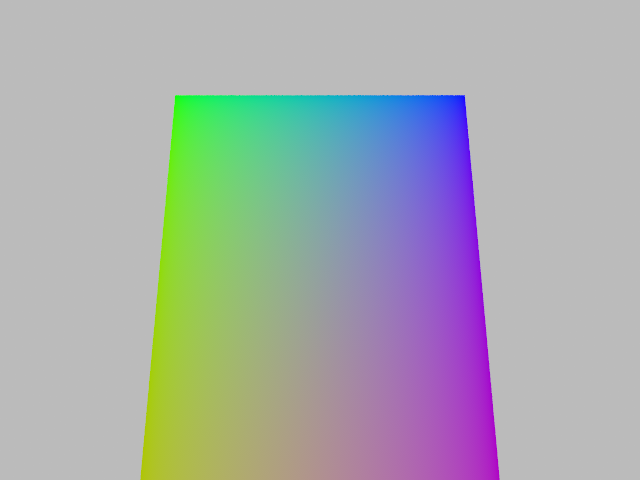
\includegraphics[width=0.3\linewidth]{imgs/hw_2_1c.png}
    \caption{References for homework 2.1.}
    \label{fig:hw_2_1}
\end{figure}

%\bibliographystyle{plain}
%\bibliography{refs}

\end{document}
